%%%%%%%%%%%%%%%%%%%%%%%%%%%%%%%%%%%%%%%%%%%%%%%%%%%%%%%%%%%%%%%%%%%%%%%%%%%%%%%%
% LaTeX Vorlage
%%%%%%%%%%%%%%%%%%%%%%%%%%%%%%%%%%%%%%%%%%%%%%%%%%%%%%%%%%%%%%%%%%%%%%%%%%%%%%%%

% Dokumentenklasse
% hier: KOMA-Script Klasse mit deutschen Features
% Eventuell in MikTeX das Paket "koma-script" nachinstallieren!
\documentclass[12pt, a4paper, DIV12]{scrartcl}

%%%%%%%%%%%%%%%%%%%%%%%%%%%%%%%%%%%%%%%%%%%%%%%%%%%%%%%%%%%%%%%%%%%%%%%%%%%%%%%%
%%% PR�AMBEL %%%%%%%%%%%%%%%%%%%%%%%%%%%%%%%%%%%%%%%%%%%%%%%%%%%%%%%%%%%%%%%%%%%
%%%%%%%%%%%%%%%%%%%%%%%%%%%%%%%%%%%%%%%%%%%%%%%%%%%%%%%%%%%%%%%%%%%%%%%%%%%%%%%%
% Deutsche Lokalisation (Umlaute etc.)
\usepackage[T1]{fontenc}
\usepackage[latin1]{inputenc} % Zeichencodierung (nicht unwichtig!)
\usepackage[ngerman]{babel}   % Deutsche Silbentrennung, etc.

% Mathematik-Erweiterungen
\usepackage{amsmath,amsfonts,amssymb}
\usepackage{siunitx}

%Bessere verbatim-Umgebung mit Syntax-Highlighting
\usepackage{listings}

% Sauberes Setzen von URLs
\usepackage{url}

% Farbige Akzente setzen
\usepackage{xcolor}

% Einbinden von Grafiken
\usepackage{graphicx}

%Einbinden von Tabellen
\usepackage{booktabs}

% PDF Optimierungen und Verlinkungen
\usepackage{hyperref}

\usepackage{amssymb}

% M�glichkit direkt mit LaTeX zu zeichnen
% \usepackage{tikz}
\usepackage{float}
\restylefloat{figure}


% Dokumentmetadaten
\title{Projektdokumentation: Roboterarm}
%\author{Jisoo Choi (3103933), Michael Vogt (4391254), Fany Bowt (4345894)}
\date{ 23.06.2017} % oder: \today


\subtitle{Grundlagen der Informatik II SOSE 2017}

%%%%%%%%%%%%%%%%%%%%%%%%%%%%%%%%%%%%%%%%%%%%%%%%%%%%%%%%%%%%%%%%%%%%%%%%%%%%%%%%
%%% DOKUMENT %%%%%%%%%%%%%%%%%%%%%%%%%%%%%%%%%%%%%%%%%%%%%%%%%%%%%%%%%%%%%%%%%%%
%%%%%%%%%%%%%%%%%%%%%%%%%%%%%%%%%%%%%%%%%%%%%%%%%%%%%%%%%%%%%%%%%%%%%%%%%%%%%%%%

\begin{document}
	

		\maketitle 	

\begin{table}[h!]
	\centering
	\begin{tabular}{c|c}
		Name  & Martikelnummer\\
		\hline
		Fany Bowt  &  4345894  \\
	
		Jisoo Choi  & 3103933   \\
		
		Michael Vogt  & 4391254   \\
	
	\end{tabular}
\end{table}

	\begin{center}
		
		
		
	\end{center}
	%Name des Versuchs: T5-Thermoelement und %Abk�hlungsgesetz\\


\tableofcontents
\newpage

\section{Beschreibung des Projekts und Funktionsweise}

Ein Arduino sollte anf�nglich 4 Mikro Servomotoren steuern, dabei befindet sich ein Servomotor bei der Konstruktion am unteren Teil des Greifarms, dieser l�sst den Arm nach rechts oder links lenken. Ein weiterer Servomotor befindet sich in der Mitte des Armes, dieser l�sst den mittleren Teils des Armes nach oben und unten steuern. Zwei Servomotoren befinden sich im oberen Teil der Konstruktion, einer der Servomotoren platziert am Greifer, um den Greifer nach oben oder unten zu bewegen und ein weiterer um die Zange zu �ffnen und zu schlie�en. 

\begin{figure}[ht]
	\centering
		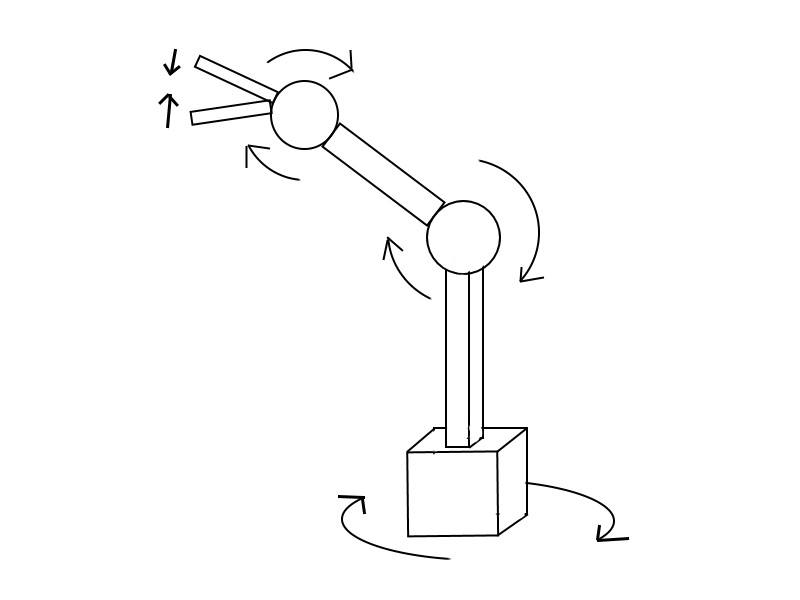
\includegraphics[width=0.43\linewidth, height=0.25\textheight]{skizze.jpg}
	\caption{Skizze vom Arm}
	\label{fig1}
\end{figure}



�ber die grafische Benutzeroberfl�che (GUI) sollte der Arm gesteuert werden. Dabei sollte mit Buttons, der jeweilige Servo und die jeweilige Richtung auszuw�hlen sein. Des Weiteren sollte die Geschwindigkeit der Servos ver�nderbar sein. \\
Wie wir mit dem Arduino kommunizieren und den Servos die Kommandos geschickt haben, wird im sp�teren Teil, beim Beschreiben des Codes genauer erl�utert. Die gesamte Kommunikation mit dem Arduino, sollte im Anschluss dann auch ohne USB Kabel funktionieren, und so wurden die gesamten Kommandos via WLAN an den Arduino gesendet. \\
Die Funktion hinter dem ganzen Projekt war, einen leicht steuerbaren Arm zu konstruieren, welcher
Sachen greifen und bewegen kann. 

\section{Der Aufbau}


Ein Arduino, welcher mit dem WLAN Shield gekoppelt ist, steuert den Roboterarm indem er Kommandos via WLAN an die einzelnen Servomotoren sendet. Um einen Servo anzusteuern sind drei Verbindungen mit dem Arduino n�tig: VCC, GND und DATA. Mittels einer speziellen Bibliothek lassen sich dann die Servos auf den 1 Grad genau ansteuern. Dabei sind die Servomotoren jedoch auf 180� mechanisch begrenzt. Es werden schlie�lich 4 Servomotoren durch den DATA-Pin von einen Arduino kontrolliert (siehe Abbildung 2). Ein weiterer Arduino dient zur Stromversorgung der Servomotoren (VCC und GND), da ansonsten das WLAN Shield nicht einwandfrei funktioniert hat, auf diesem Arduino ist kein Code hochgeladen worden. 



\begin{figure}[ht]
	\centering
		\includegraphics[width=0.89\linewidth, height=0.26\textheight]{schaltbild.png}
	\caption{Schaltbild}
	\label{Schaltbild}
\end{figure}


Die Arme wurden aus Holz ausgeschnitten. Anschlie�end konnten die Servos mit kleinen Schrauben am Holz befestigt werden. Eine gr��ere Holzplatte dient als Unterlage. 
Sehr wichtig war es, dass der Arm ein Ausgleichsgewicht besitzt da sonst der Servo zu stark belastet wird, sodass der Arm nicht hochgehoben werden kann. 

\begin{figure}[ht]
	\centering
	\includegraphics[width=1.0\linewidth, height=0.26\textheight]{aufbau}
	\caption{Aufbau}
	\label{aufbau}
\end{figure}



\section{Arduino/C Code-Beschreibung}


\subsection{Setup}

Mittels der Bibliohtek servo.h lassen sich die servos sehr simpel ansteuern. 
Dazu m�ssen zun�chst Variablen als Servos geklariert werden (siehe Abbildung 3 Zeile 7-10) und daraufhin auf welchen Pin (Zeile 11-14). Diese Pins sind dann an DATA anzuschlie�en. Im Setup wird dann mit dem Befehl servo.attach($servo\_pin$) der jeweilige Servo einem Pin zugewiesen.

\begin{figure}[ht]
	\centering
	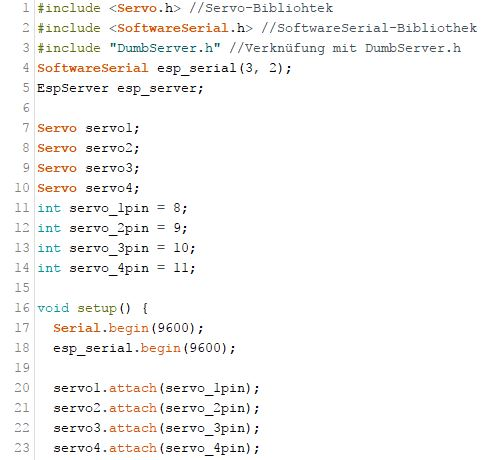
\includegraphics[width=0.4\linewidth, height=0.25\textheight]{setup}
	\caption{If-funktion mit dem Auslesen der Kommandos via WLAN}
	\label{setup}
\end{figure}

\subsection{Steuerungsfunktionen}

In unserem C Code haben wir zuerst vier Funktionen erstellt. Eine dient dazu den jeweiligen Servomotor nach links zu bewegen und eine Andere, um ihn nach rechts zu bewegen. Die anderen beiden Funktionen, die sogenannten Spezial-Funktionen, bewirken, dass Servo  Nr. 2 und Nr. 3 immer die Summe aus 180� bilden. Dadurch bleibt der mittlere Teil des Armes, siehe Abbildung 1, immer Senkrecht stehen, dies l�sst sich nach oben sowie nach unten steuern.

\begin{figure}[ht]
	\centering
		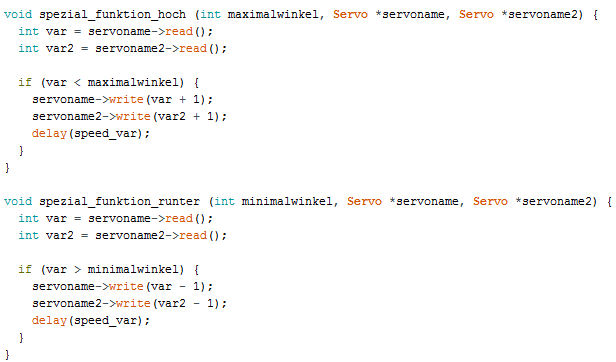
\includegraphics[width=0.6\linewidth, height=0.25\textheight]{spezialfunktion.png}
	\label{spezialfunktion}
	\caption{Bewegungsfunktionen}
\end{figure}

\subsection{Die Loop}

Damit der Arduino sein empfangenes Kommando ausf�hrt, wird mit der Variable $python\_button\_var$ ein Switch-Cases integriert. Switch-Cases funktioniert nur mit Zahlen bzw. Integern. Darum m�ssen die in Python gesendeten Buchstaben zun�chst in den If-Funktionen zu Integern umge�ndert werden, damit anschlie�end die Cases benutzt werden k�nnen. 

\begin{figure}[ht]
	\centering
	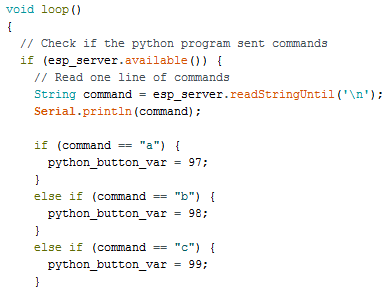
\includegraphics[width=0.45\linewidth, height=0.25\textheight]{if.png}
	\caption{If-funktion mit dem Auslesen der Kommandos via WLAN}
	\label{IF}
\end{figure}


Neben den Richtungen k�nnen wir mit Switch Cases auch die Geschwindigkeit der Servomotoren ver�ndern, indem das Delay gr��er oder kleiner gesetzt wird f�r die Variable $speed\_var$.  (Siehe Abbilung 6, Case 49-54)

\begin{figure}[ht]
	\centering
	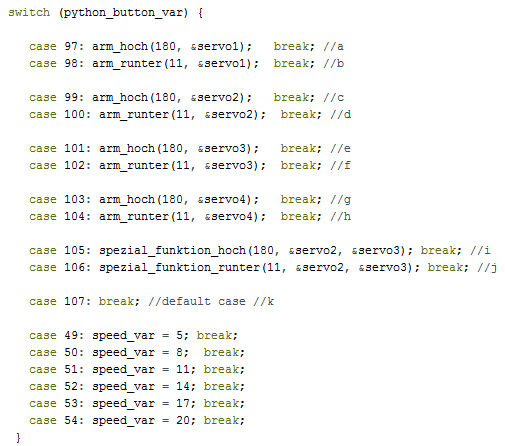
\includegraphics[width=0.6\linewidth, height=0.3\textheight]{switch.png}
	\caption{Die switch-case}
	\label{Switch}
\end{figure}

\subsection{WLAN-Empfang}

In unserem Code lassen wir den Arduino etwas �ber das WLAN empfangen, indem wir die DumbServer.h, sowie DumbServer.cpp eingebaut haben. Diese erlauben uns eine Verbidnung mit dem WLAN-Shield ESP8266 herzustellen. \\
Um mit dem Python Programm in Verbindung zu treten, ben�tigen wir die IP Adresse und den richtigen Port. Den Port teilen wir dem Python und dem Arduino Programm selber zu, die IP Adresse erfahren wir durch unser Arduinprogramm, sobald wir den seriellen Monitor �ffnen und der Server gestartet ist. \\
Das genaue Kommando welches wir empfangen und auslesen, tun wir mit dem oberen Teil des Codes in Abbildung 6.


\section{Python Code und GUI}

\begin{figure}[ht]
	\centering
	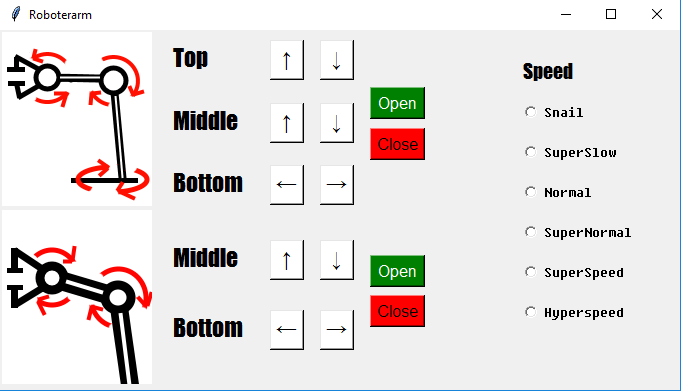
\includegraphics[width=0.8\textwidth, height=205px]{GUI.png}
	\caption{Die mit Tkinter erstellte GUI}
	\label{GUI}
\end{figure}


\end{document}
